\documentclass[tikz,border=5pt]{standalone}
\usepackage{fontspec}
\setmainfont{Times New Roman}
\usepackage{unicode-math}
\setmathfont{Cambria Math}
\usetikzlibrary{shapes.geometric,shapes.misc,positioning,fit,backgrounds,arrows.meta,calc}

\begin{document}
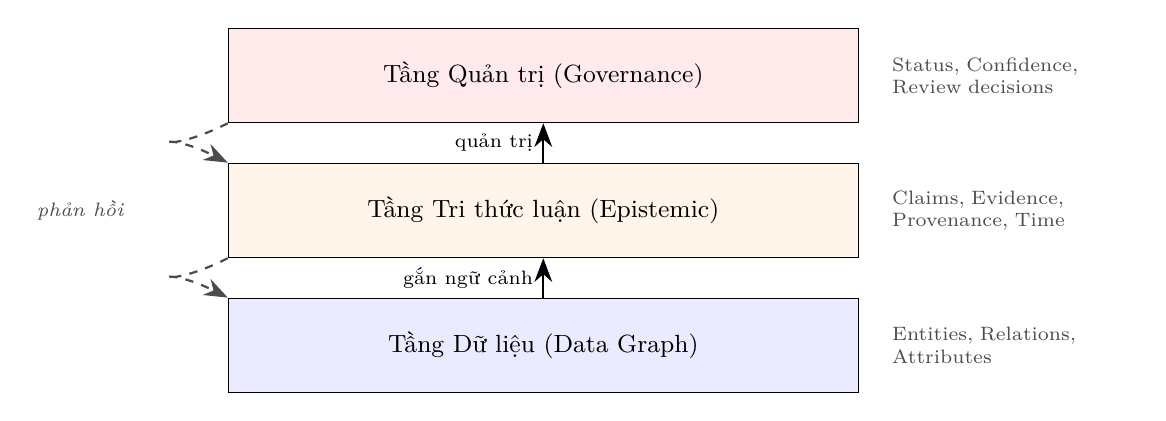
\begin{tikzpicture}[
    layer/.style={rectangle, draw, minimum width=8cm, minimum height=1.2cm, align=center, font=\small},
    arrow/.style={-{Stealth[length=3mm]}, thick},
    note/.style={font=\scriptsize, text=gray!60!black, align=left, text width=3cm},
]

% Three layers stacked
\node[layer, fill=red!8] (gov) {Tầng Quản trị (Governance)};
\node[layer, fill=orange!8, below=0.5cm of gov] (epi) {Tầng Tri thức luận (Epistemic)};
\node[layer, fill=blue!8, below=0.5cm of epi] (data) {Tầng Dữ liệu (Data Graph)};

% Layer contents
\node[note, right=0.3cm of gov] {Status, Confidence,\\Review decisions};
\node[note, right=0.3cm of epi] {Claims, Evidence,\\Provenance, Time};
\node[note, right=0.3cm of data] {Entities, Relations,\\Attributes};

% Arrows between layers
\draw[arrow] (data.north) -- node[left, font=\scriptsize] {gắn ngữ cảnh} (epi.south);
\draw[arrow] (epi.north) -- node[left, font=\scriptsize] {quản trị} (gov.south);

% Feedback arrows
\draw[arrow, dashed, gray!60!black] (gov.south west) .. controls +(-1,-0.5) and +(-1,0.5) .. (epi.north west);
\draw[arrow, dashed, gray!60!black] (epi.south west) .. controls +(-1,-0.5) and +(-1,0.5) .. (data.north west);
\node[font=\scriptsize\itshape, text=gray!60!black, left=1.2cm of epi] {phản hồi};

\end{tikzpicture}
\end{document}
